\chapter[Solução Proposta] {Solução Proposta}

A proposta deste projeto envolve a integração dos cinco cursos de engenharia que são lecionados no campus UnB - Gama, com o intuito de resolver os problemas apresentados acima. A proposta inicial de solução se baseia no desenvolvimento de uma biblioteca automatizada, com capacidade de receber um comando do usuário de requerimento do livro, recolher o livro da estante e entregá-lo em cima de uma plataforma, onde o usuário irá poder pegá-lo. Além disso o robô será capaz de fazer o processo contrário, recolher o livro da plataforma e guardá-lo na estante, atualizando o sistema em tempo real.

Este capítulo tem como objetivo apresentar o detalhamento das soluções propostas dos sub-sistemas da \textit{Bibliotech}.

\section{Requisitos do Sistema}
A construção do sistema \textit{Bibliotech} visa atender os seguintes requisitos: 
\begin{figure}[!htb]
     \centering
     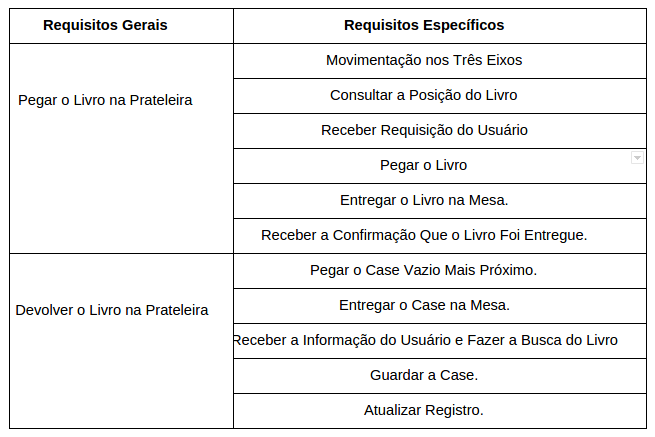
\includegraphics[scale=1]{images/requisitos.png}
     \caption{Requisitos do Produto}
     \label{Requisitos do Produto}
\end{figure}